\documentclass[a4paper]{article}

\def\npart {III}
\def\nterm {Michaelmas}
\def\nyear {2017}
\def\nlecturer {R.\ D.\ Shah}
\def\ncourse {Modern Statistical Methods}
\def\nofficial {https://www.statslab.cam.ac.uk/~rds37/modern_statistical_methods}
% Imports
\ifx \nextra \undefined
  \usepackage[pdftex,
    hidelinks,
    pdfauthor={Dexter Chua},
    pdfsubject={Cambridge Maths Notes: Part \npart\ - \ncourse},
    pdftitle={Part \npart\ - \ncourse},
  pdfkeywords={Cambridge Mathematics Maths Math \npart\ \nterm\ \nyear\ \ncourse}]{hyperref}
  \title{Part \npart\ - \ncourse}
\else
  \usepackage[pdftex,
    hidelinks,
    pdfauthor={Dexter Chua},
    pdfsubject={Cambridge Maths Notes: Part \npart\ - \ncourse\ (\nextra)},
    pdftitle={Part \npart\ - \ncourse\ (\nextra)},
  pdfkeywords={Cambridge Mathematics Maths Math \npart\ \nterm\ \nyear\ \ncourse\ \nextra}]{hyperref}

  \title{Part \npart\ - \ncourse \\ {\Large \nextra}}
\fi

\author{Lectured by \nlecturer \\\small Notes taken by Dexter Chua}
\date{\nterm\ \nyear}

\usepackage{alltt}
\usepackage{amsfonts}
\usepackage{amsmath}
\usepackage{amssymb}
\usepackage{amsthm}
\usepackage{booktabs}
\usepackage{caption}
\usepackage{enumitem}
\usepackage{fancyhdr}
\usepackage{graphicx}
\usepackage{mathtools}
\usepackage{microtype}
\usepackage{multirow}
\usepackage{pdflscape}
\usepackage{pgfplots}
\usepackage{siunitx}
\usepackage{tabularx}
\usepackage{tikz}
\usepackage{tkz-euclide}
\usepackage[normalem]{ulem}
\usepackage[all]{xy}

\pgfplotsset{compat=1.12}

\pagestyle{fancyplain}
\lhead{\emph{\nouppercase{\leftmark}}}
\ifx \nextra \undefined
  \rhead{
    \ifnum\thepage=1
    \else
      \npart\ \ncourse
    \fi}
\else
  \rhead{
    \ifnum\thepage=1
    \else
      \npart\ \ncourse\ (\nextra)
    \fi}
\fi
\usetikzlibrary{arrows}
\usetikzlibrary{decorations.markings}
\usetikzlibrary{decorations.pathmorphing}
\usetikzlibrary{positioning}
\usetikzlibrary{fadings}
\usetikzlibrary{intersections}
\usetikzlibrary{cd}

\newcommand*{\Cdot}{\raisebox{-0.25ex}{\scalebox{1.5}{$\cdot$}}}
\newcommand {\pd}[2][ ]{
  \ifx #1 { }
    \frac{\partial}{\partial #2}
  \else
    \frac{\partial^{#1}}{\partial #2^{#1}}
  \fi
}

% Theorems
\theoremstyle{definition}
\newtheorem*{aim}{Aim}
\newtheorem*{axiom}{Axiom}
\newtheorem*{claim}{Claim}
\newtheorem*{cor}{Corollary}
\newtheorem*{defi}{Definition}
\newtheorem*{eg}{Example}
\newtheorem*{fact}{Fact}
\newtheorem*{law}{Law}
\newtheorem*{lemma}{Lemma}
\newtheorem*{notation}{Notation}
\newtheorem*{prop}{Proposition}
\newtheorem*{thm}{Theorem}

\renewcommand{\labelitemi}{--}
\renewcommand{\labelitemii}{$\circ$}
\renewcommand{\labelenumi}{(\roman{*})}

\let\stdsection\section
\renewcommand\section{\newpage\stdsection}

% Strike through
\def\st{\bgroup \ULdepth=-.55ex \ULset}

% Maths symbols
\newcommand{\bra}{\langle}
\newcommand{\ket}{\rangle}

\newcommand{\N}{\mathbb{N}}
\newcommand{\Z}{\mathbb{Z}}
\newcommand{\Q}{\mathbb{Q}}
\renewcommand{\H}{\mathbb{H}}
\newcommand{\R}{\mathbb{R}}
\newcommand{\C}{\mathbb{C}}
\newcommand{\Prob}{\mathbb{P}}
\renewcommand{\P}{\mathbb{P}}
\newcommand{\E}{\mathbb{E}}
\newcommand{\F}{\mathbb{F}}
\newcommand{\cU}{\mathcal{U}}
\newcommand{\RP}{\mathbb{RP}}
\newcommand{\CP}{\mathbb{CP}}

\newcommand{\ph}{\,\cdot\,}

\DeclareMathOperator{\sech}{sech}
\DeclareMathOperator{\cosech}{cosech}
\DeclareMathOperator{\cosec}{cosec}

\DeclareMathOperator{\covol}{covol}
\DeclareMathOperator{\vol}{vol}

\let\Im\relax
\let\Re\relax
\DeclareMathOperator{\Im}{Im}
\DeclareMathOperator{\Re}{Re}
\DeclareMathOperator{\im}{im}
\DeclareMathOperator{\image}{image}
\DeclareMathOperator{\Ann}{Ann}

\DeclareMathOperator*{\res}{res}
\DeclareMathOperator{\Res}{Res}
\DeclareMathOperator{\Ind}{Ind}

\DeclareMathOperator{\tr}{tr}
\DeclareMathOperator{\diag}{diag}
\DeclareMathOperator{\rank}{rank}
\DeclareMathOperator{\card}{card}
\DeclareMathOperator{\spn}{span}
\DeclareMathOperator{\adj}{adj}

\DeclareMathOperator{\erf}{erf}
\DeclareMathOperator{\erfc}{erfc}

\DeclareMathOperator{\ord}{ord}
\DeclareMathOperator{\Sym}{Sym}

\DeclareMathOperator{\sgn}{sgn}
\DeclareMathOperator{\orb}{orb}
\DeclareMathOperator{\stab}{stab}
\DeclareMathOperator{\ccl}{ccl}

\DeclareMathOperator{\lcm}{lcm}
\DeclareMathOperator{\hcf}{hcf}

\DeclareMathOperator{\Int}{Int}
\DeclareMathOperator{\id}{id}

\DeclareMathOperator{\betaD}{beta}
\DeclareMathOperator{\gammaD}{gamma}
\DeclareMathOperator{\Poisson}{Poisson}
\DeclareMathOperator{\binomial}{binomial}
\DeclareMathOperator{\multinomial}{multinomial}
\DeclareMathOperator{\Bernoulli}{Bernoulli}
\DeclareMathOperator{\like}{like}

\DeclareMathOperator{\var}{var}
\DeclareMathOperator{\cov}{cov}
\DeclareMathOperator{\bias}{bias}
\DeclareMathOperator{\mse}{mse}
\DeclareMathOperator{\corr}{corr}

\DeclareMathOperator{\otp}{otp}
\DeclareMathOperator{\dom}{dom}

\DeclareMathOperator{\Root}{Root}
\DeclareMathOperator{\supp}{supp}
\DeclareMathOperator{\rel}{rel}
\DeclareMathOperator{\Hom}{Hom}
\DeclareMathOperator{\Aut}{Aut}
\DeclareMathOperator{\Gal}{Gal}
\DeclareMathOperator{\Mat}{Mat}
\DeclareMathOperator{\End}{End}
\DeclareMathOperator{\Char}{char}
\DeclareMathOperator{\ev}{ev}
\DeclareMathOperator{\St}{St}
\DeclareMathOperator{\Lk}{Lk}
\DeclareMathOperator{\disc}{disc}
\DeclareMathOperator{\Isom}{Isom}
\DeclareMathOperator{\length}{length}
\DeclareMathOperator{\energy}{energy}
\DeclareMathOperator{\area}{area}
\DeclareMathOperator{\Syl}{Syl}
\DeclareMathOperator{\cl}{cl}
\DeclareMathOperator{\fix}{fix}

\newcommand{\GL}{\mathrm{GL}}
\newcommand{\SL}{\mathrm{SL}}
\newcommand{\PGL}{\mathrm{PGL}}
\newcommand{\PSL}{\mathrm{PSL}}
\newcommand{\PSU}{\mathrm{PSU}}
\newcommand{\Or}{\mathrm{O}}
\newcommand{\SO}{\mathrm{SO}}
\newcommand{\U}{\mathrm{U}}
\newcommand{\SU}{\mathrm{SU}}

\renewcommand{\d}{\mathrm{d}}
\newcommand{\D}{\mathrm{D}}

\tikzset{->/.style = {decoration={markings,
                                  mark=at position 1 with {\arrow[scale=2]{latex'}}},
                      postaction={decorate}}}
\tikzset{<-/.style = {decoration={markings,
                                  mark=at position 0 with {\arrowreversed[scale=2]{latex'}}},
                      postaction={decorate}}}
\tikzset{<->/.style = {decoration={markings,
                                   mark=at position 0 with {\arrowreversed[scale=2]{latex'}},
                                   mark=at position 1 with {\arrow[scale=2]{latex'}}},
                       postaction={decorate}}}
\tikzset{->-/.style = {decoration={markings,
                                   mark=at position #1 with {\arrow[scale=2]{latex'}}},
                       postaction={decorate}}}
\tikzset{-<-/.style = {decoration={markings,
                                   mark=at position #1 with {\arrowreversed[scale=2]{latex'}}},
                       postaction={decorate}}}

\tikzset{circ/.style = {fill, circle, inner sep = 0, minimum size = 3}}
\tikzset{mstate/.style={circle, draw, blue, text=black, minimum width=0.7cm}}

\definecolor{mblue}{rgb}{0.2, 0.3, 0.8}
\definecolor{morange}{rgb}{1, 0.5, 0}
\definecolor{mgreen}{rgb}{0.1, 0.4, 0.2}
\definecolor{mred}{rgb}{0.5, 0, 0}

\def\drawcirculararc(#1,#2)(#3,#4)(#5,#6){%
    \pgfmathsetmacro\cA{(#1*#1+#2*#2-#3*#3-#4*#4)/2}%
    \pgfmathsetmacro\cB{(#1*#1+#2*#2-#5*#5-#6*#6)/2}%
    \pgfmathsetmacro\cy{(\cB*(#1-#3)-\cA*(#1-#5))/%
                        ((#2-#6)*(#1-#3)-(#2-#4)*(#1-#5))}%
    \pgfmathsetmacro\cx{(\cA-\cy*(#2-#4))/(#1-#3)}%
    \pgfmathsetmacro\cr{sqrt((#1-\cx)*(#1-\cx)+(#2-\cy)*(#2-\cy))}%
    \pgfmathsetmacro\cA{atan2(#2-\cy,#1-\cx)}%
    \pgfmathsetmacro\cB{atan2(#6-\cy,#5-\cx)}%
    \pgfmathparse{\cB<\cA}%
    \ifnum\pgfmathresult=1
        \pgfmathsetmacro\cB{\cB+360}%
    \fi
    \draw (#1,#2) arc (\cA:\cB:\cr);%
}
\newcommand\getCoord[3]{\newdimen{#1}\newdimen{#2}\pgfextractx{#1}{\pgfpointanchor{#3}{center}}\pgfextracty{#2}{\pgfpointanchor{#3}{center}}}

\def\Xint#1{\mathchoice
   {\XXint\displaystyle\textstyle{#1}}%
   {\XXint\textstyle\scriptstyle{#1}}%
   {\XXint\scriptstyle\scriptscriptstyle{#1}}%
   {\XXint\scriptscriptstyle\scriptscriptstyle{#1}}%
   \!\int}
\def\XXint#1#2#3{{\setbox0=\hbox{$#1{#2#3}{\int}$}
     \vcenter{\hbox{$#2#3$}}\kern-.5\wd0}}
\def\ddashint{\Xint=}
\def\dashint{\Xint-}


\DeclareMathOperator*\argmin{argmin}
\begin{document}
\maketitle
{\small
\setlength{\parindent}{0em}
\setlength{\parskip}{1em}

The remarkable development of computing power and other technology now allows scientists and businesses to routinely collect datasets of immense size and complexity. Most classical statistical methods were designed for situations with many observations and a few, carefully chosen variables. However, we now often gather data where we have huge numbers of variables, in an attempt to capture as much information as we can about anything which might conceivably have an influence on the phenomenon of interest. This dramatic increase in the number variables makes modern datasets strikingly different, as well-established traditional methods perform either very poorly, or often do not work at all.

Developing methods that are able to extract meaningful information from these large and challenging datasets has recently been an area of intense research in statistics, machine learning and computer science. In this course, we will study some of the methods that have been developed to analyse such datasets. We aim to cover some of the following topics.

\begin{itemize}
 \item Kernel machines: the kernel trick, the representer theorem, support vector machines, the hashing trick.
 \item Penalised regression: Ridge regression, the Lasso and variants.
 \item Graphical modelling: neighbourhood selection and the graphical Lasso. Causal inference through structural equation modelling; the PC algorithm.
 \item High-dimensional inference: the closed testing procedure and the Benjamini--Hochberg procedure; the debiased Lasso
\end{itemize}

\subsubsection*{Pre-requisites}
Basic knowledge of statistics, probability, linear algebra and real analysis. Some background in optimisation would be helpful but is not essential.
}
\tableofcontents

\section{Introduction}
In recent years, there has been a rather significant change in what sorts of data we have to handle and what questions we ask about them. Hence, new methods have to be developed to analyze them. For example, in classical statistics, we often have very few variables, and a very large data set. However, nowadays, we have a lot of different variables, and perhaps not as much data. This is known as high-dimensional statistics.

Of course, we cannot cover absolutely everything, and we are going to cover $4$ different topics of different size:
\begin{itemize}
  \item Kernel machines
  \item The Lasso and its extensions
  \item Graphical modeling and causal inference
  \item Multiple testing and high-dimensional inference
\end{itemize}
The four topics are rather disjoint, and they draw on different mathematical skills.

\section{Classical statistics}
This is a course on \emph{modern} statistical methods. Before we study methods, we give a brief summary of what we are \emph{not} going to talk about, namely classical statistics.

So suppose we are doing regression. We have some \term{predictors} $x_i \in \R^p$ and \term{responses} $Y_i \in \R$, and we hope to find a model that describes $Y$ as a function of $x$. For convenience, define the vectors
\[
  X = \begin{pmatrix} x_1^T \\ \vdots \\ x_n^T\end{pmatrix},\quad
  Y = \begin{pmatrix} Y_1^T \\ \vdots \\ Y_n^T\end{pmatrix}.
\]
The linear model then assumes there is some $\beta^0 \in \R^p$ such that
\[
  Y = X \beta^0 + \varepsilon,
\]
where $\varepsilon$ is some (hopefully small) error random variable. Our goal is then to estimate $\beta^0$ given the data we have.

If $X$ has full column rank, so that $X^TX$ is invertible, then we can use \term{ordinary least squares} to estimate $\beta^0$, with estimate
\[
  \hat{\beta}^{OLS} = \argmin_{\beta \in \R^p} \|Y - x \beta\|_2^2 = (X^TX)^{-1} X^TY.
\]
This assumes nothing about $\varepsilon$ itself, but if we assume that $\E \varepsilon = 0$ and $\var (\mathcal{E}) = \sigma^2 I$, then this estimate satisfies
\begin{itemize}
  \item $\E_\beta \hat{\beta}^{OLS} = (X^T X)^{-1} X^T X \beta^0 = \beta^0$
  \item $\var_\beta(\hat{\beta}^{OLS}) = (X^T X^{-1}) X^T \var(\varepsilon) X (X^T X)^{-1} = \sigma^2 (X^T X)^{-1}$.
\end{itemize}
In particular, this is an unbiased estimator. Even better, this is the best linear unbiased estimator. More precisely, the Gauss--Markov theorem says any other linear estimator $\tilde{\beta} = AY$ has $\var(\tilde{\beta}) - \var(\hat{\beta}^{OLS})$ positive semi-definite.

Of course, ordinary least squares is not the only way to estimate $\beta^0$. Another common method for estimating parameters is maximum likelihood estimation, and this works for more general models than linear regression. For people who are already sick of meeting likelihoods, this will be the last time we meet likelihoods in this course.

Suppose we want to estimate a parameter $\theta$ via knowledge of some data $Y$. We assume $Y$ has density $f(y; \theta)$. We define the \term{log-likelihood} by
\[
  \ell(\theta) = \log f(Y, \theta).
\]
The \term{maximum likelihood estimator} then maximize $\ell(\theta)$ over $\theta$ to get $\hat{\theta}$.

Similar to ordinary least squares, there is a theorem that says maximum likelihood estimation is the ``best''. To do so, we introduce the \term{Fisher information matrix}. This is a family of $d \times d$ matrices indexed by $\theta$, defined by
\[
  I_{jk}(\theta) = - E_\theta\left[\frac{\partial^2}{\partial \theta_j \partial \theta_j} \ell(\theta)\right].
\]
The relevant theorem is
\begin{thm}[Cram\'er--Rao bound]\index{Cram\'er--Rao bound}
  If $\tilde{\theta}$ is an unbiased estimator for $\theta$, then $\var(\tilde{\theta}) - I^{-1}(\theta)$ is positive semi-definite.

  Moreover, asymptotically, as $n \to \infty$, the maximum likelihood estimator is unbiased and achieves the Carm\'er--Rao bound.
\end{thm}

Another wonderful fact about the maximum likelihood estimator is that asymptotically, it is normal distributed, and so it is something we unerstand well.

This might seem very wonderful, but there are a few problems here. The results we stated are asymptotic, but what we actually see in real life is that as $n \to \infty$, the value of $p$ also increases. In these contexts, the asymptotic property doesn't tell us much. Another issue is that these all talk about unbiased estimators. In a lot of situations of interest, it turns out biased methods do much much better than these methods we have.

Another thing we might be interested is that as $n$ gets large, we might want to use more complicated models that simple parametric models, as we have much more data to mess with. This is not something ordinary least squares provides us with.

\section{Kernel machines}
We are going to start a little bit slowly, and think about our linear model $Y = X\beta^0 + \varepsilon$, where $\E(\varepsilon) = 0$ and $\var(\varepsilon) = \sigma^2 I$. Ordinary least squares is an unbiased estimator, so let's look at biased estimators.

For a biased estimator, $\tilde{\beta}$, we should not study the variance, but
\begin{align*}
  \E[(\tilde{\beta} - \beta^0)(\tilde{\beta} - \beta^0)^T]
  &= \E(\tilde{\beta} - \E \tilde{\beta} + E \tilde{\beta} - \beta^0)(\tilde{\beta} - \E \tilde{\beta} + E \tilde{\beta} - \beta^0)^T \\ &= \var(\tilde{\beta})+ (\E \tilde{\beta} - \beta^0)(\E \tilde{\beta} - \beta^0)^T
\end{align*}
The first term is, of course, just the variance, and the second is the squared bias. So the point is that if we pick a clever biased estimator with a tiny variance, then this might do better than unbiased estimators with large variance.

\subsection{Ridge regression}
This is probably one of the oldest methods we are going to discuss in this course, introduced in around 1970. The idea of Ridge regression, as well as the Lasso, is that we want to shrink our estimator a bit, so that the variance will be smaller, even though we have introduced a bias. An extreme case is when we always estimate $\beta$ by $0$, in which case there is no variance but a (potentially) large bias.

The \term{Ridge regression} solves
\[
  (\hat{\mu}^R_\lambda, \hat{\beta}^R_\lambda) = \argmin_{(\mu, \beta) \in \R \times \R^p} \{ \|Y - \mu \mathbf{1} - X \beta\|_2^2 + \lambda \| + \lambda \|\beta\|_2^2\},
\]
where $\mathbf{1}$ is a vector of all $1$'s. Here $\lambda \geq 0$ is a tuning parameter, and it controls how much we penalize a large choice of $\beta$.

We explicitly have an intercept term. Usually, we introduce this by adding a column of $1$'s in $X$. But here we want to separate that out, since we do not want give a penalty for large $\mu$.

For example, if the parameter is temperature, then if we decide to measure in degrees Celsius rather than Kelvins, where we add a linear shift to all terms, we don't want the resulting $\hat{\mu}, \hat{\beta}$ to change. More precisely, if we make the modification
\[
  Y' = c\mathbf{1} + Y,
\]
then we have
\[
  \hat{\mu}^R_\lambda(Y') = \hat{\mu}_\lambda^R(Y) + c.
\]
Note also that this formula makes sense only if each entry in $\beta$ have the same order of magnitude, or else the penalty will only have a significant effect on the terms of large magnitude. Standard practice is to subtract from each column of $X$ its mean, and then scale it to have $\ell_2$ norm $\sqrt{n}$. The actual number is not important here, but it will in the case of the Lasso.

In example sheet 1, we will show that this gives
\begin{align*}
  \hat{\mu}_\lambda^R &= \bar{Y} = \frac{1}{n} \sum Y_i\\
  \hat{\beta}^R_\lambda &= (X^T X + \lambda I)^{-1} X^T Y.
\end{align*}
A first thing to note that we can always pick $\lambda$ such that the matrix $(X^T X + \lambda I)$ is invertible. In particular, this can work even if we have more parameters than data points.
\begin{thm}
  Suppose $\rank(X) = p$. Then for $\lambda > 0$ sufficiently small, we have that
  \[
    \E(\hat{\beta}^{OLS} - \beta^0)(\hat{\beta}^{OLS} - \beta^0)^T - \E(\hat{\beta}^{R}_\lambda - \beta^0)(\hat{\beta}^{R}_\lambda - \beta^0)^T \tag{$*$}
  \]
  is positive definite.
\end{thm}
The ``sufficiently small'' depends on $\beta_0$ and $\sigma^2$.

The proof is a computation.
\begin{proof}
  We know that the first term is just $\sigma^2(X^T X)^{-1}$. The right-hand-side has a variance term and a bias term. We first look at the bias:
  \begin{align*}
    \E [\hat{\beta} - \beta^0] &= (X^T X + \lambda I)^{-1} X^T X \beta^0 - \beta^0\\
    &= (X^T X + \lambda I)^{-1}(X^T X + \lambda I - \lambda I) \beta^0- \beta^0\\
    &= \lambda (X^T X + \lambda I)^{-1} \beta^).
  \end{align*}
  We can also compute the variance
  \[
    \var(\hat{\beta}) = \sigma^2(X^T X + \lambda I)^{-1} X^T X (X^T X + \lambda I)^{-1}.
  \]
  Note that both terms appearing in the squared error look like
  \[
    (X^T X + \lambda I)^{-1}\text{something}(X^T X + \lambda I)^{-1}.
  \]
  So let's try to write $\sigma^2 (X^T X)^{-1}$ in this form. Note that
  \begin{align*}
    (X^T X)^{-1} &= (X^T X + \lambda I)^{-1} (X^T X + \lambda I) (X^T X)^{-1} (X^T X + \lambda I) (X^T X + \lambda I)^{-1}\\
    &= (X^T X + \lambda I)^{-1}(X^T X + 2 \lambda I + \lambda^2 (X^T X)^{-1}) (X^T X + \lambda I)^{-1}.
  \end{align*}
  Thus, we can write $(*)$ as
  \begin{align*}
    &\hphantom{ {} = {} }(X^T X + \lambda I)^{-1} \Big( \sigma^2(X^T X + 2 \lambda I + \lambda^2(X^T X)^{-1}) - \sigma^2 X^T X - \lambda^2 \beta^0 (\beta^0)^T\Big) (X^T X + \lambda I)^{-1}\\
    &= \lambda (X^T X + \lambda I)^{-1} \Big( 2 \sigma^2 I + \lambda(X^T X)^{-1} - \lambda \beta^0 (\beta^0)^T\Big) (X^T X + \lambda I)^{-1}
  \end{align*}
  Since $\lambda > 0$, this is positive definite iff
  \[
    2 \sigma^2 I + \sigma^2 \lambda (X^T X)^{-1} - \lambda \beta^0 (\beta^0)^T
  \]
  is positive definite, which is true for $0 < \lambda < \frac{2\sigma^2}{\|\beta^0\|_2^2}$.
\end{proof}
While this is nice, this is not really telling us much, because we don't know how to pick the correct $\lambda$. It also doesn't tell us when we should expect a big improvement from Ridge regression.

To understand this better ,we need to use the \emph{singular value decomposition}
\subsection{The singular value decomposition (SVD)}

\begin{thm}[Singular value decomposition]\index{singular value decomposition}\index{SVD}
  Let $X \in \R^{n \times p}$ be any matrix. Then it has a \emph{singular value decomposition} (SVD)
  \[
    \underset{n \times p}{X} = \underset{n \times n}{U} D\underset{n \times p}D \underset{p \times p}{V^T},
  \]
  where $U, V$ are orthogonal matrices, and $D_{nn} \leq D_{22} \leq \cdots \leq D_{mm} \geq 0$, where $m = \min (n, p)$, and all other entries are zero.
\end{thm}

When $n > p$, there is an alternative version where $U$ is an $n \times p$ matrix with orthogonal columns, and $D$ is a $p \times p$ diagonal matrix. This is done by replacing $U$ by its first $p$ columns and $D$ by its first $p$ rows. This is known as the \term{thin singular value decomposition}\index{thin SVD}. In this case, $U^T U = I_p$ but $UU^T$ is not the identity.

Let's now apply try to understand Ridge regressions a little better. Suppose $n > p$. Then using the thin SVD, the fitted values from ridge regression are
\begin{align*}
  X \hat{\beta}_\lambda^R &= X (X^T X + \lambda I)^{-1} X^T Y\\
  &= UDV^T (VD^2 V^T + \lambda I)^{-1} VDU^T Y.
\end{align*}
We now note that $VD^2 V^T + \lambda I = V(D^2 + \lambda I)V^T$, since $V$ is still orthogonal. We then have
\[
  (V (D^2 + \lambda I)V^T)^{-1} = V(D^2 + \lambda I)^{-1} V^T
\]
Since $D^2$ and $\lambda I$ are both diagonal, it is easy to compute their inverses as well. We then have
\[
  X\hat{\beta}_\lambda^R = UD^2 (D^2 + \lambda I)^{-1} U^T Y = \sum_{j = 1}^p U_j \frac{D_{jj}^2}{ D_{jj}^2 + \lambda} U_j^T Y
\]
Here $U_j$ refers to the $j$th column of $U$.

Now note that the columns of $U$ form an orthonormal basis for the column space of $X$. If $\lambda = 0$, then this is just a fancy formula for the projection of $Y$ onto the column space of $X$. Thus, what this formula is telling us is that we look at this projection, look at the coordinates in terms of the basis given by the columns of $U$, and scale accordingly.

We can now concretely see the effect of our $\lambda$. The shrinking depends on the size of $D_{jj}$, and the larger $D_{jj}$ is, the less shrinking we do. What is special about the columns of $U$ is that they are exactly the normalized principal components of $X$.

Take $u \in \R^p$, $\|u\|_2 = 1$. The sample variance of $Xu \in \R^n$ is
\[
  \frac{1}{n} \|Xu\|_2^2 = \frac{1}{n} u^T X^T X u = \frac{1}{n} u^T VD^2 V^t u.
\]
We write $w = V^T u$. Then $\|w\|_2 = 1$ since $V$ is orthogonal. We then have
\[
  \frac{1}{n} \|Xu\|_2^2 = \frac{1}{n} w^T D^2 w = \frac{1}{n} \sum_j w_j^2 D_{jj^2} \leq \frac{1}{n} D_{11}^2,
\]
and this bound is achieved when $w = e_1$. So we need $u = V e_1 = V_1$. Thus, $V_1$ gives the coefficients of the linear combination of columns of $X$ that has largest sample variance subject to the coefficient vector having $\ell_2$ norm $1$. The result is then
\[
  X V_1 = U DV^T V_1 = U_1 D_{11}.
\]
We can extend this to a description of the other columns of $U$, which is done in the example sheet. Roughly, the subsequent principle components obey the same optimality conditions with the added constraint of being orthogonal to all earlier principle components.

The conclusion is that Ridge regression works best if $\E Y$ lies in the space spanned by the large principal components of $X$. % insert example?

\subsection{\texorpdfstring{$v$}{v}-fold cross-validation}
In practice, if we are given a data set, how do we know what $\lambda$ we should pick? $v$-fold cross-validation is a very general technique to do so, which allows us to pick a regression method from a variety of options. We are explaining our method in terms of Ridge regression, where our regression methods are parametrized by a single parameter $\lambda$. However, our method in fact allows us to compare vastly different regression methods.

Suppose we are given data $(Y_i, x_i)_{i = 1}^n$ and a new data point $(Y^*, x^*) \in \R \times \R^p$ are iid, and $Y^*$ is not observed. We may want to pick $\lambda$ to minimize the following quantity:
\[
  \E \left\{ (Y^* - (x^*)^T \hat{\beta}_\lambda^R(X, Y))^2 \mid X, Y \right\}.
\]
It is difficult to actually do this, and so an easier target to minimize is the expected prediction error
\[
  \E\left[\E \left\{ (Y^* - (x^*)^T \hat{\beta}_\lambda^R(\tilde{X}, \tilde{Y}))^2 \mid \tilde{X}, \tilde{Y} \right\}\right]
\]
One thing to note about this is that we are thinking of $\tilde{X}$ and $\tilde{Y}$ as arbitrary data sets of size $n$, as opposed to the one we have actually got.

This might be a more tractable problem, since we are not working with our actual data set, but general data sets.

The method of cross-validation estimates this by splitting the data into $v$ folds.
\begin{center}
  \begin{tikzpicture}
    \draw (0, 0) rectangle +(3, 1);
    \draw (0, 5) rectangle +(3, 1);

    \draw [dashed] (0, 1) -- (0, 5);
    \draw [dashed] (3, 1) -- (3, 5);

    \node at (4, 0.5) {$(X^{(1)}, Y^{(1)})$};
    \node at (6, 0.5) {$A_1$};

    \node at (4, 5.5) {$(X^{(v)}, Y^{(v)})$};
    \node at (6, 5.5) {$A_v$};
  \end{tikzpicture}
\end{center}
$A_i$ is called the \term{observation indices}, which is the set of all indices $i$ so that the $i$th data point lies in the $i$th fold.

We let $(X^{(-k)}, Y^{(-k)})$ be all data except that in the $k$th fold. We define
\[
  CV(\lambda) = \frac{1}{n} \sum_{k = 1}^v \sum_{i \in A_k} (Y_i - x_I^T \hat{\beta}_\lambda^R (X^{(-k)}, Y^{(-k)}))^2
\]
We write $\lambda_{CV}$ for the minimizer of this, and pick $\hat{\beta}^R_{\lambda_{CV}}(X, Y)$ as our estimate. This tends to work very will in practice.

But we can ask ourselves --- why do we have to pick a single $\lambda$ to make the estimate? We can instead average over a range of different $\lambda$. Suppose we have computed $\hat{\beta}_\lambda^R$ on a grid of $\lambda$-values $\lambda_1 > \lambda_2 > \cdots > \lambda_L$. Our plan is to take a good weighted average of the $\lambda$. Concretely, we want to minimize
\[
  \frac{1}{n} \sum_{k = 1}^v \sum_{i \in A_k} \left(Y_i - \sum_{i = 1}^L w_i x_i^T \hat{\beta}_{\lambda_i}^R (X^{(-k)}, Y^{(-k)})\right)^2
\]
over $w \in [0, \infty)^L$. This is known as \term{stacking}. This tends to work better than simply $v$-fold cross-validation. Indeed, it must --- cross-validation is just a special case where we restrict $w_i$ to be zero in all but one entries. Of course, one disadvantage of this approach is that after solving this minimization problem, whenever we want to make our prediction, we need to compute a lot of different $\hat{\beta}_{\lambda}^R$ in order to do so.

\subsection{The kernel trick}
We start with a very simple observation. An alternative way of writing the fitted values from Ridge regression is
\[
  (X^T X + \lambda I) X^T = X^T(X^T + \lambda I).
\]
One should be careful that the $\lambda I$ are different matrices on both sides, as they have different dimensions. Inverting the matrices, we have
\[
  X^T(XX^T + \lambda I)^{-1} = (X^T X + \lambda I)^{-1} X^T.
\]
We can multiply the right-hand-side by $Y$ to obtain the $\hat{\beta}$ by Ridge regression, and multiply on the left to obtain the fitted values. So we have
\[
  XX^T(XX^T + \lambda I)^{-1}Y = X (X^T X + \lambda I)^{-1} X^T Y = X \hat{\beta}^R_\lambda.
\]
Note that $X^T X$ is a $p \times p$ matrix, and takes $O(np^2)$ time to compute. On the other hand, $XX^T$ is an $n \times n$ matrix, and takes $O(n^2 p)$ time to compute. If $p \gg n$, then this would be faster to compute.

The key point to make is that the fitted values from Ridge regression only depends on $K = XX^T$ (and $Y$). Why is this important?

Suppose we believe we have a quadratic signal
\[
  Y_i = x_i^T \beta + \sum_{k, \ell} x_{ik} x_{i\ell} \theta_{k\ell} + \varepsilon_i
\]
Of course, we can do Ridge regression, as long as we add the products $x_{ik} x_{i\ell}$ as predictors. But this requires $O(p^2)$ many predictors. Even if we use the $XX^T$ way, this has a cost of $O(n^2 p^2)$, and if we were really naive, it would require $O(np^4)$ operations.

We need to do better than this. The idea is that we might be able to compute $k$ directly. Consider
\[
  (1 + x_i^T x_j)^2 = 1 + 2 x_i^T x_j + \sum_{k, \ell} x_{ik} x_{i\ell} x_{jk}x_{j\ell}.
\]
This is equal to the inner product between vectors of the form
\[
  (1, \sqrt{2} x_{i1}, \ldots, \sqrt{2}x_{ip}, x_{i1} x_{i1}, \ldots, x_{i1} x_{ip}, x_{i2} x_{i1}, \ldots, x_{ip} x_{ip})\tag{$*$} % arrange this better
\]
If we set $K_{ij} = (1 + x_i^T x_j)^2$ and form $K(K + \lambda I)^{-1} Y$, this is equivalent to forming ridge regression with $(*$) as our predictors. Note that here we don't scale our columns to have the same $\ell_2$ norm.

This is pretty interesting, because computing this is only $O(n^2p)$. We managed to kill a factor of $p$ in this computation.

More generally, since the Ridge fitted values only depends on inner products between different observations, if we want to try to fit some other complicated model, instead of fitting non-linear models by first mapping each $\{x_i\} \mapsto \phi(x_i) \in \R^d$ using some ``feature map'' $\phi$, we can instead aim to directly compute
\[
  \bra \phi(x_i), \phi(x_j)\ket = k(x_i, x_j).
\]
But we can also try to go in the other direction. We don't need to know $\phi$ itself, but we simply have to find some appropriate $k(x_i, x_j)$, which should be some ``similarity measure'' between $x_i$ and $x_j$, and then set $K_{ij} = k(x_i, x_j)$.

\subsection{Kernels}
We'll aim to characterize the similarity measures $k: \mathcal{X} \times \mathcal{X} \to \R$ for which there exists a feature map $\phi: \mathcal{X} \to \mathcal{H}$, where $\mathcal{H}$ is a real inner product space, with% use $\mathcal{X}$
\[
  k(x, x') = \bra \phi(x), \phi(x')\ket.
\]
We are being slightly more general than we were last time, where we allow $\mathcal{H}$ to be fancy.

Recall that an inner product space is a real vector space $\mathcal{H}$ endowed with a map $\bra \ph, \ph \ket: \mathcal{H} \times \mathcal{H} \to \R$ and obeys
\begin{itemize}
  \item Symmetry: $\bra u, v \ket = \bra v, u\ket$
  \item Linearity: If $a, b \in \R$, then $\bra au + bw, v\ket = a \bra u, v\ket + b \bra w, v\ket$.
  \item Positive definiteness: $\bra u, u \ket \geq 0$ with $\bra u, u \ket = 0$ iff $u = 0$.
\end{itemize}

\begin{defi}[Positive-definite kernel]\index{positive-definite kernel}\index{kernel}
  A \emph{positive-definite kernel} (or simply \emph{kernel}) is a symmetric map $k: \mathcal{X} \times \mathcal{X} \to \R$ such that for all $n \in \N$ and $x_1, \ldots, x_n \in \mathcal{X}$, the matrix $K \in \R^n \times \R^n$ with entries
  \[
    K_{ij} = k(x_i, x_j)
  \]
  is positive semi-definite.
\end{defi}
Note that our definition of ``positive semi-definite'' includes being symmetric.

It turns out the Cauchy--Schwarz inequality still holds for positive semi-definite matrices
\begin{prop}[Cauchy--Schwarz inequality]\index{Cauchy--Schwarz inequality}
  We have
  \[
    k(x, x')^2 \leq k(x, x) k(x', x')
  \]
\end{prop}

\begin{proof}
  The matrix
  \[
    \begin{pmatrix}
      k(x, x) & k(x, x')\\
      k(x', x) & k(x', x')
    \end{pmatrix}
  \]
  has to be positive semi-definite by assumption, and expanding out, we are done.
\end{proof}

\begin{prop}
  $k$ defined by
  \[
    k(x, x') = \bra \phi(x), \phi(x')\ket
  \]
  is a kernel.
\end{prop}

\begin{proof}
  Let $x_1, \ldots, x_n \in \mathcal{X}$, and $\alpha \in \R^n$. Consider
  \begin{align*}
    \sum_{i, j} \alpha_i k(x_i, x_j) \alpha_jh &= \sum_{i, j} \alpha_i \bra \phi(x_i), \phi(x_j)\ket\\
    &= \left\bra \sum_i \alpha_i \phi(x_i), \sum_j \alpha_j \phi(x_j)\right\ket\\
    &\geq 0
  \end{align*}
  since the inner product is positive definite.
\end{proof}

It would be nice to have a way to construct new kernels from old kernels.
\begin{eg}
  Suppose $k_1, k_2, \ldots, k_n$ are kernels. Then
  \begin{itemize}
    \item If $\alpha_1, \alpha_2 \geq 0$, then $\alpha_1 k_1 + \alpha_2 k_2$ is a kernel.

    If $\lim_{m \to \infty} k_m(x, x') \equiv k(x, x')$ exists, then $k$ is a kernel.
    \item The pointwise product $k_1k_2$ is a kernel (where $(k_1 k_2)(x, x') = k_1(x, x') k_2(x, x')$)
  \end{itemize}
\end{eg}
Proofs are left as an exercise on the example sheet.

\begin{eg}
  The \term{linear kernel} is $k(x, x') = x^T x'$. To see this, we see that this is given by the feature map $\phi = \id$ and taking the standard inner product on $\R^p$.
\end{eg}

\begin{eg}
  The \term{polynomial kernel} is $k(x, x') = (1 + x^T x')^d$ for all $d \in \N$.

  We saw this last time with $d = 2$. This is a kernel since both $1$ and $x^T x'$ are kernels, and sums and products preserve kernels.
\end{eg}

\begin{eg}
  The \term{Gaussian kernel} is
  \[
    k(x, x') = \exp\left(- \frac{\|x- x'\|^2_2}{2\sigma^2}\right).
  \]
  The quantity $\sigma$ is known as the \term{bandwidth}.% $\sigma$ or $\sigma^2$?

  To show that it is a kernel, we decompose
  \[
    \|x - x'\|_2^2 = \|x\|_2^2 + \|x'\|_2^2 - 2 x^T x'.
  \]
  We define
  \[
    k_1(x, x') = \exp\left(-\frac{\|x\|_2^2}{2\sigma^2}\right)\exp\left(-\frac{\|x'\|_2^2}{2\sigma^2}\right).
  \]
  This is a kernel by taking $\phi(\ph) = \exp\left(-\frac{\|\ph\|_2^2}{2\sigma^2}\right)$.

  Next, we can define
  \[
    k_2(x, x') = \exp\left(\frac{x^T x'}{\sigma^2}\right) = \sum_{r = 0}^\infty \frac{1}{r!} \left(\frac{x^T x'}{\sigma^2}\right)^r.
  \]
  We see that this is the infinite linear combination of powers of kernels, hence is a kernel.

  Thus, it follows that $k = k_1 k_2$ is a kernel.

  Note also that any feature map giving this $k$ must take values in an infinite dimensional inner product space. Roughly speaking, this is because we have arbitrarily large powers of $x$ and $x'$ in the expansion of $k$.
\end{eg}

\begin{eg}
  The \term{Sobolev kernel} is defined as follows: we take $\mathcal = [0, 1]$, and let
  \[
    k(x, x') = \min(x, x').
  \]
  This is the covariance function of Brownian motion, so must be a kernel.
\end{eg}

\begin{eg}
  The \term{Jaccard similarity} is defined as follows: Take $\mathcal{X}$ to be the set of all subsets of $\{1, \ldots, p\}$. For $x, x' \in \mathcal{X}$, define
  \[
    k(x, x') =
    \begin{cases}
      \frac{|x \cap x'|}{|x \cup x'|} & x \cup x' \not= \emptyset\\
      1 & \text{otherwise}
    \end{cases}.
  \]
\end{eg}

\subsection{Reproducing kernel Hilbert spaces}
\begin{thm}[Moore--Aronszajn theorem]\index{Moore--Aronszajn theorem}
  For every kernel $k: \mathcal{X} \times \mathcal{X} \to \R$, there exists an inner product space $\mathcal{H}$ and a feature map $\phi: \mathcal{X} \to \mathcal{H}$ such that
  \[
    k(x, x') = \bra \phi(x), \phi(x')\ket.
  \]
\end{thm}
This is not actually the full Moore--Aronszajn theorem, but a simplified version of it.

\begin{proof}
  Let $\mathcal{H}$ denote the vector space of functions $f: \mathcal{X} \to \R$ of the form
  \[
    f(\ph) = \sum_{i = 1}^n \alpha_i k(\cdot, x_i)\tag{$*$}
  \]
  for some $n \in \N$, $\alpha_1, \ldots, \alpha_n \in \R$ and $x_1, \ldots, x_n \in \mathcal{X}$. If
  \[
    g(\ph) = \sum_{i = 1}^m \beta_j k(\ph, x_j') \in \mathcal{H},
  \]
  then we tentatively define the inner product of $f$ and $g$ by
  \[
    \bra f, g\ket = \sum_{i = 1}^n \sum_{j = 1}^m \alpha_i \beta_j k(x_i, x_j').
  \]
  We have to check that this is an inner product, but even before that, we need to check that this is well-defined, since $f$ and $g$ can be represented in the form $(*)$ in multiple ways. To do so, simply observe that
  \[
    \sum_{i = 1}^n \sum_{j = 1}^m \alpha_i \beta_j k(x_i, x_j') = \sum_{i = 1}^n \alpha_i g(x_i) = \sum_{j = 1}^m \beta_j f(x_j').\tag{$\dagger$}
  \]
  The first equality shows that the definition of our inner product does not depend on the representation of $g$, while the second equality shows that it doesn't depend on the representation of $f$.

  To show this is an inner product, note that it is clearly symmetric and bilinear. To show it is positive definite, note that we have
  \[
    \bra f, f \ket = \sum_{i = 1}^n \sum_{j = 1}^m \alpha_i k(x_i, x_j) \alpha_j \geq 0
  \]
  since the kernel is positive semi-definite. It remains to check that if $\bra f, f\ket = 0$, then $f = 0$ as a function. To this end, note the important reproducing property: by $(\dagger)$, we have
  \[
    \bra k(\ph, x), f\ket = f(x).
  \]
  This says $k(\cdot, x)$ represents the evaluation-at-$x$ linear functional.

  In particular, we have
  \[
    f(x)^2 = \bra k(\ph, x), f\ket^2 \leq \bra k(\ph, x), k(\ph, x)\ket \bra f, f\ket = 0.
  \]
  Here we used the Cauchy--Schwarz inequality, which, if you inspect the proof, does not require positive definiteness, just positive semi-definiteness. So it follows that $f \equiv 0$. Thus, we know that $\mathcal{H}$ is indeed an inner product space.

  We now have to construct a feature map. Define $\phi: \mathcal{X} \to \mathcal{H}$ by
  \[
    \phi(x) = k(\ph, x).
  \]
  Then we have already observed that
  \[
    \bra \phi(x), \phi(x')\ket = \bra k(\ph, x), k(\ph, x')\ket = k(x, x'),
  \]
  as desired.
\end{proof}

How can we boost this theorem up to its full strength, where we say there is a ``unique'' inner product space with such a feature map. Of course, it will not be unique unless we impose appropriate quantifiers, since we can just throw in some random elements into $\mathcal{H}$.

Recall (or learn) from functional analysis that any inner product space $\mathcal{B}$ is a normed space, with norm
\[
  \|f\|^2 = \bra f,f \ket_\mathbf{B}.
\]
We say sequence $(f_m)$ in a normed space $\mathcal{B}$ if $\|f_m - f_n\|_\mathcal{B} \to 0$ as $n, m \to \infty$. An inner product space is \emph{complete}\index{complete inner product space} if every Cauchy sequence has a limit (in the space), and a complete inner product space is called a \term{Hilbert space}.

One important property of a Hilbert space $\mathcal{B}$ is that if $V$ is a closed subspace of $\mathcal{B}$, then every $f \in \mathcal{B}$ has a unique representation as $f = v + w$, where $v \in V$ and
\[
  w \in V^\perp = \{u \in \mathcal{B}: \bra u, y\ket = 0 \forall y \in V\}.
\]
By adding limits of Cauchy sequences to $\mathcal{H}$, we can obtain a Hilbert space. Indeed, if $(f_m)$ is Cauchy in $\mathcal{H}$, then
\[
  |f_m(x) - f_n(x)| \leq k^{1/2}(x, x) \|f_m - f_n\|_{\mathcal{H}} \to 0
\]
as $m, n \to \infty$. Since every Cauchy sequence in $\R$ converges (i.e.\ $\R$ is complete), it makes sense to define a limiting function
\[
  f(x) = \lim_{n \to \infty} f_n(x),
\]
and it can be shown that after augmenting $\mathcal{H}$ with such limits, we obtain a Hilbert space. In fact, it is a special type of Hilbert space.

\begin{defi}[Reproudcing kernel Hilbert space (RKHS)]\index{reproducing kernel Hilbert space}\index{RKHS}
  A Hilbert space $\mathcal{B}$ of functions $f: \mathcal{X} \to \R$ is a reproducing kernel Hilbert space if for each $x \in \mathcal{X}$, there exists a $k_x \in \mathcal{B}$ such that
  \[
    \bra k_x, f\ket = f(x)
  \]
  for all $x \in \mathcal{B}$.

  The function $k: \mathcal{X} \times \mathcal{X} \to \R$ given by
  \[
    k(x, x') = \bra k_x, k_x'\ket = k_x(x') = k_{x'}(x)
  \]
  is called the \term{reproducing kernel} associated with $\mathcal{B}$.
\end{defi}
By the Riesz representation theorem, this condition is equivalent to saying that pointwise evaluation is continuous.

We know the reproducing kernel associated with an RKHS is a positive-definite kernel, and the Moore--Aronszajn theorem can be extended to show that to each kernel $k$, there is a unique representing kernel Hilbert space $\mathcal{H}$ and feature map $\phi: \mathcal{X} \to \mathcal{H}$ such that $k(x, x') = \bra \phi(x), \phi(x')\ket$.

\begin{eg}
  Take the linear kernel
  \[
    k(x, x') = x^T x'.
  \]
  By definition, we have
  \[
    \mathcal{H} = \{f:\R^p \to \R \mid f(x) = \sum_{i = 1}^n \alpha_i x_i^T x\}
  \]
  for some $n \in \N$, $x_1, \ldots, x^n \in \R^p$. We then see that this is equal to
  \[
    \mathcal{H} = \{f: \R^p \to \R \mid f(x) = \beta^T x\text{ for some }\beta \in \R^p\},
  \]
  and if $f(x) = \beta^T x$, then $\|f\|_{\mathcal{H}}^2 = k(\beta, \beta) = \|\beta\|^2_2$.
\end{eg}

\begin{eg}
  Take the Sobolev kernel, where $\mathcal{X} = [0, 1]$ and $k(x, x') = \min(x, x')$. Then $\mathcal{H}$ includes all linear combinations of functions of the form $x \mapsto \min(x, x')$, where $x' \in [0, 1]$, and their pointwise limits. These functions look like
  \begin{center}
    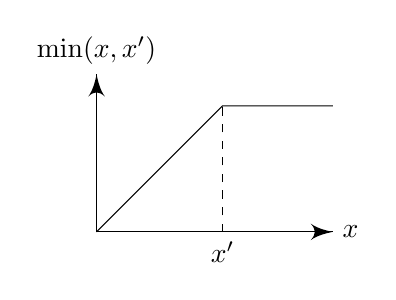
\begin{tikzpicture}
      \draw [->] (0, 0) -- (3, 0) node [right] {$x$};
      \draw [->] (0, 0) -- (0, 2) node [above] {$\min(x, x')$};

      \draw (0, 0) -- (1.6, 1.6) -- (3, 1.6);

      \draw [dashed] (1.6, 0) node [below] {$x'$} -- (1.6, 1.6);
    \end{tikzpicture}
  \end{center}
  Since we allow arbitrary linear combinations of these things and pointwise limits, this gives rise to a large class of functions. In particular, this includes all Lipschitz functions that are $0$ at the origin.

  In fact, the resulting space is a Sobolev space, with the norm given by% check this
  \[
    \|f\| = \left(\int_0^1 f'(x)^2 \;\d x \right)^{1/2}.
  \]
  For example, if we take $f = \min (\ph, x)$, then by definition we have
  \[
    \|\min(\ph, x)\|_\mathcal{H}^2 = \min(x, x) = x,
  \]
  whereas the formula we claimed gives
  \[
    \int_0^x 1^2 \;\d t = x.
  \]
  The proof is quite tricky.
\end{eg}

In general, it is difficult to understand the RKHS, but if we can do so, this provides a lot of information on what we are regularizing in the kernel trick.

\subsection{The representer theorem}
Let's now try to understand what exactly we are doing when we do Ridge regression with a kernel $k$.

Note that for the linear kernel, the $L^2$ norm $\|\beta\|_2^2$ corresponds exactly to the norm in the RKHS $\|f\|_{\mathcal{H}}^2$. Thus, an alternative way of expressing ridge regression is
\[
  \argmin_{f \in \mathcal{H}} \left\{\sum_{i = 1}^n (Y_i - f(x_i))^2 + \lambda \|f\|_{\mathcal{H}}^2 \right\},\tag{$*$}
\]
where $\mathcal{H}$ is the RKHS of the linear kernel. We might guess that it is true in complete generality.

\begin{thm}[Representer theorem]\index{representer theorem}
  Let $\mathcal{H}$ be an RKHS with reproducing kernel $k$. Let $c$ be an arbitrary loss function and $J: [0, \infty) \to \R$ any strictly increasing function. Then $\hat{f}$ minimizes
  \[
    Q_1(f) = c(Y, x_1, \ldots, x_n, f(x_1), \ldots, f(x_n)) + J(\|f\|_{\mathcal{H}}^2)
  \]
  over all functions $f \in \mathcal{H}$ iff
  \[
    \hat{f}(\ph) = \sum_{i = 1}^n \hat{\alpha}_i k(\ph, x_i)
  \]
  and $\hat{\alpha} \in \R^n$ minimizes
  \[
    Q_2(\alpha) = c(Y, x_1, \ldots, x_n, K\alpha) + J(\alpha^T K \alpha),
  \]
  over $\alpha \in \R^n$ (with $K_{ij}(x_i, \ldots, x_j)$).
\end{thm}
For an arbitrary $c$, the second function can be quite hard to optimize. But in the case of Ridge regression, this tells us that $(*)$ is equivalent to minimizing
\[
  \|Y - K\alpha\|_2^2 + \lambda \alpha^T K \alpha,
\]
and we know that this is given by
\[
  K \hat{\alpha} = K(K + \lambda I)^{-1} Y.
\]
\begin{proof}
  Suppose $\hat{f}$ minimizes $Q_1$. We can then write
  \[
    \hat{f} = u + v
  \]
  where $u \in V = \spn\{k(\ph, x_i): i = 1, \ldots ,n\}$ and $v \in V^\perp$. Then
  \[
    \hat{f}(x_i) = \bra f, k(\ph, x_i)\ket = \bra u + v, k(\ph, x_i)\ket = \bra u, k(\ph, x_i)\ket = u(x_i).
  \]
  So we know that
  \[
    c(Y, x_1, \ldots, x_n, f(x_1), \ldots, f(x_n)) = c(Y, x_1, \ldots, x_n, u(x_1), \ldots, u(x_n)).
  \]
  Meanwhile,
  \[
    \|f\|^2_{\mathcal{H}} = \|u + v\|^2_{\mathcal{H}} = \|u\|^2_{\mathcal{H}} + \|v\|^2_{\mathcal{H}},
  \]
  using the fact that $u$ and $v$ are orthogonal. So we know
  \[
    J(\|f\|_{\mathcal{H}}^2 ) \geq J(\|u\|_{\mathcal{H}}^2)
  \]
  with equality iff $v = 0$. Hence $Q_1(f) \geq Q_1(u)$ with equality iff $v = 0$, and so we must have $v = 0$ by optimality.

  Thus, we know that the optimizer in fact lies in $V$, and then the formula of $Q_2$ just expresses $Q_1$ in terms of $\alpha$.
\end{proof}

\subsection{Kernel ridge regression}
Consider a model
\[
  Y_i = f^0(x_i) + \varepsilon_i
\]
for $i = 1, \ldots, n$, and assume $\E \varepsilon = 0$ and $\var(\varepsilon) = \sigma^2 I$. This is analogous to the ridge regression setting, but now we have a more general function $f^0$.

We assume $f^0 \in \mathcal{H}$, where $\mathcal{H}$ is an RKHS with reproducing kernel $k$. We assume $\|f^0\|^2_{\mathcal{H}} \leq 1$. There is no loss in generality by assuming this, since we can always achieve this by scaling the norm.

Let $K$ be the kernel matrix $K_{ij} = k(x_i, x_j)$ with eigenvalues $d_1 \geq d_2 \geq \cdots \geq d_n \geq 0$. Define
\[
  \hat{f}_\lambda = \argmin_{f \in \mathcal{H}} \left\{ \sum_{i = 1}^n (Y_i - f(x_i))^2 + \lambda \|f\|_\mathcal{H}^2\right\}.
\]
\begin{thm}
  We have
  \begin{align*}
    \frac{1}{n} \sum_{i = 1}^n \E(f^0(x_i) - \hat{f}_\lambda (x_i))^2 &\leq \frac{\sigma^2}{n} \sum_{i = 1}^n \frac{d_i^2}{(d_i + \lambda)^2} + \frac{\lambda}{4n}\\
    &\leq \frac{\sigma^2}{n} \frac{1}{\lambda} \sum_{i = 1}^n \min \left(\frac{d_i}{r}, \lambda\right) + \frac{\lambda}{4n}.
  \end{align*}
\end{thm}
Given a data set, we can compute the eigenvalues $d_i$, and thus we can compute this error bound.

\begin{proof}
  We know from the representer theorem that
  \[
    (\hat{f}_\lambda (x_i), \ldots, \hat{f}_\lambda (x_n))^T = K(K + \lambda I)^{-1} Y.
  \]
  Also,
  \[
    (f^0(x_1), \ldots, f^0(x_n))^T = K \alpha
  \]
  for some $\alpha \in \R^n$ by an example sheet question. Moreover,
  \[
    1 \geq \|f^0\|_{\mathcal{H}}^2 \geq \alpha^T K \alpha.
  \]
  So we are now in matrix world, and everything is much more familiar.

  Consider the eigendecomposition of $K = UDU^T$, where $U$ is orthogonal, $D_{ii} = d_i$ and $D_{ij} = 0$ for $i \not= j$. Then we have
  \begin{align*}
    \E \sum_{i = 1}^n (f^0(x_i) - \hat{f}_\lambda (x_i))^2 &= \E\|K\alpha - K(K + \lambda I)^{-1} (k\alpha + \varepsilon)\|_2^2\\
    \intertext{Noting that $K\alpha= (K + \lambda I)(K + \lambda I)^{-1} K\alpha$, we obtain}
    &= \E \norm{\lambda (K + \lambda I)^{-1} K\alpha - K(K + \lambda I)^{-1} \varepsilon}_2^2\\
    &= \underbrace{\lambda^2 \norm{(K + \lambda I)^{-1} K\alpha\|_2^2}}_{\mathrm{(I)}} + \underbrace{\E \norm{K(K + \lambda I)^{-1} \varepsilon}_2^2}_{\mathrm{(II)}}.
  \end{align*}
  At this stage, we can throw in the eigendecomposition of $K$ to write (I) as
  \begin{align*}
    \mathrm{(I)} &= \lambda^2 \norm{(UDU^T + \lambda I)^{-1} UDU^T \alpha }_2^2\\
    &= \lambda^2 \|U (D + \lambda I)^{-1} \underbrace{D U^T \alpha}_{\theta} \|_2^2\\
    &= \sum_{i = 1}^n \theta_i^2 \frac{\lambda^2}{(d_i + \lambda)^2}
  \end{align*}
  Now we have
  \[
    \alpha^T K \alpha = \alpha^T U DU^T \alpha = \alpha^T U DD^+ DU^T,
  \]
  where $D^+$ is diagonal and
  \[
    D_{ii}^+ =
    \begin{cases}
      d_i^{-1} & d_i > 0\\
      0 & \text{otherwise}
    \end{cases}.
  \]
  We can then write this as
  \[
    \alpha^T K \alpha = \sum_{d_i > 0} \frac{\theta_i^2}{d_i}.
  \]
  The key thing we know about this is that it is $\leq 1$.

  Note that by definition of $\theta_i$, we see that if $d_i = 0$, then $\theta_i = 0$. So we can write
  \[
    \mathrm{(II)} = \sum_{i: d_i \geq 0} \frac{\theta_i^2}{d_i} \frac{d_i \lambda^2}{(d_i + \lambda)^2} \leq \lambda \max_{i = 1, \ldots, n} \frac{d_i \lambda}{(d_i + \lambda)^2}
  \]
  by H\"older's inequality with $(p, q) = (1, \infty)$. Finally, use the inequality that
  \[
    (a + b)^2 \geq 4ab
  \]
  to see that we have
  \[
    \mathrm{(I)} \leq \frac{\lambda}{4}.
  \]
  So we are left with (II), which is a bit easier. Using the trace trick, we have
  \begin{align*}
    \mathrm{(II)} &= \E \varepsilon^T (K + \lambda I)^{-1} K^2 (K + \lambda I)^{-1} \varepsilon\\
    &= \E \tr \left(K (K + \lambda I)^{-1} \varepsilon \varepsilon^T (K + \lambda I)^{-1} K\right)\\
    &= \tr \left(K (K + \lambda I)^{-1} \E(\varepsilon \varepsilon^T) (K + \lambda I)^{-1} K\right)\\
    &= \sigma^2 \tr \left(K^2(K + \lambda I)^{-2}\right)\\
    &= \sigma^2 \tr \left(UD^2 U^T (UDU^T + \lambda I)^{-2}\right)\\
    &= \sigma^2 \tr \left(D^2 (D + \lambda I)^{-2}\right)\\
    &= \sigma^2 \sum_{i = 1}^n \frac{d_i^2}{(d_i + \lambda)^2}.
  \end{align*}
  Finally, writing $\frac{d_i^2}{(d_i + \lambda)^2} = \frac{d_i}{\lambda} \frac{d_i \lambda}{(d_i + \lambda)^2}$, we have
  \[
    \frac{d_i^2}{(d_i + \lambda)^2} \leq \min \left(1, \frac{d_i}{4 \lambda}\right),
  \]
  and we have the second bound.
\end{proof}
How can we interpret this? If we look at the formula, then we see that we can have good benefits if the $d_i$'s decay quickly, and the exact values of the $d_i$ depend only on the choice of $x_i$. So suppose the $x_i$ are random and idd and independent of $\varepsilon$. Then the entire analysis is still valid by conditioning on $x_1, \ldots, x_n$.

We define $\hat{\mu}_i = \frac{d_i}{n}$, and $\lambda_n = \frac{\lambda}{n}$. Then we can rewrite our result to say
\[
  \frac{1}{n} \E \sum_{i = 1}^n (f^0(x_i) - \hat{f}_\lambda (x_i))^2 \leq \frac{\sigma^2}{\lambda_n} \frac{1}{n} \sum_{i = 1}^n \E \min\left(\frac{\hat{\mu}_i}{4}, \lambda_n\right) + \frac{\lambda_n}{4} \equiv \E \delta_n(\lambda_n).
\]
We want to relate this more directly to the kernel somehow. Given a density $p(x)$ on $\mathcal{X}$, \term{Mercer's theorem} guarantees the following eigenexpansion
\[
  k(x, x') = \sum_{j = 1}^\infty \mu_j e_j(x) e_j(x'),
\]
where the eigenvalues $\mu_j$ and eigenfunctions $e_j$ obey
\[
  \mu_j e_j(x') = \int_{\mathcal{X}} k(x, x') e_j(x) p(x)\;\d x
\]
and
\[
  \int_{\mathcal{X}} e_k(x) e_j(x) p(x)\;\d x = \mathbf{1}_{j = k}.
\]
One can show that
\[
  \frac{1}{n} \E \sum_{i = 1}^n \min \left(\frac{\hat{\mu}_i}{4}, \lambda_n\right) \leq \frac{1}{n} \sum_{i = 1}^\infty \sum_{i = 1}^\infty \min\left(\frac{\mu_i}{4}, \lambda_n\right)
\]
up to some absolute constant factors (like $\sqrt{2}$). For a particular density $p(x)$ of the input space, we can try to solve the integral equation to figure out what the $\mu_j$'s are, and we can find the expected bound.

When $k$ is the Sobolev kernel and $p(x)$ is the uniform density, then it turns out we have
\[
  \frac{\mu_j}{4} = \frac{1}{\pi^2(2j - 1)^2}.
\]
By drawing a picture, we see that we can bound $\sum_{i = 1}^\infty \min \left(\frac{\mu_i}{4} , \lambda_n\right)$ by
\[
  \sum_{i = 1}^\infty \min \left(\frac{\mu_i}{4} , \lambda_n\right) \leq \int_0^\infty \lambda_n \wedge \frac{1}{\pi^2(2j - 1)^2}\;\d j \leq \frac{\sqrt{\lambda_n}}{\pi} + \frac{\lambda_n}{2}.
\]
So we find that
\[
  \E(\delta_n(\lambda_n)) = O \left(\frac{\sigma^2}{n \lambda_n^{1/2}} + \lambda_n\right).
\]
We can then find the $\lambda_n$ that minimizes this, and we see that we should pick
\[
  \lambda_n \sim \left(\frac{\sigma^2}{n}\right)^{2/3},
\]
which gives an error rate of $\sim \left(\frac{\sigma^2}{n}\right)^{2/3}$.

\subsection{Other kernel machines}
Recall that the representer theorem was much more general than what we used it for. We could apply it to any loss function. In particular, we can apply it to classification problems. For example, we might want to predict whether an email is a spam. In this case, we have $Y \in \{-1, 1\}^n$.

\subsubsection*{The support vector machine}
Suppose $\{x_i\}_{y_i = 1}$ and $\{x_i\}_{i: Y_i = -1}$ are separable by a hyperplane through the origin. So there exists $\beta \in \R^p$ (the normal vector) with $y_i x_I^T \beta> 0$ for all $i$. Moreover, it would be nice if we can maximize the minimum distance between any of the points and the hyperplane defined by $\beta$. This is given by
\[
  \max \frac{y_i x_i^T \beta}{\|\beta\|_2}.
\]
Thus, we can formulate our problem as
\begin{center}
  Maximize $M$ among $\beta \in \R^p, M \geq 0$ subject to $\frac{y_i x_i^T \beta}{\|\beta\|_2} \geq M$.
\end{center}
This optimization problem gives the hyperplane that maximizes the \emph{margin} between the two classes.

Let's think about the more realistic case where we cannot completely separate the two sets. We then want to impose a penalty for each point on the wrong side, and attempt to minimize the distance.

There are two options. We can use the penalty
\[
  \lambda \sum_{i = 1}^n \left(M - \frac{Y_i x_i^T \beta}{\|\beta\|_2}\right)_+
\]
where $(t)_+ = t \mathbf{1}_{t \geq 0}$. Another option is to take
\[
  \lambda \sum_{i = 1}^n \left(1 - \frac{Y_i x_i^T \beta}{M \|\beta\|_2}\right)+
\]
which is perhaps more natural, since we are measuring things in unit of length $M$. It turns out it is this second option that leads to a tractable convex optimization problem. Using this, our problem becomes
\[
  \max_{M \geq 0, \beta \in \R^p} \left(M - \lambda \sum_{i = 1}^n \left(1 - \frac{Y_i x_i^T \beta}{M \|\beta\|_2}\right)_+\right).
\]
Since the objective function is invariant to any positive scaling of $\beta$, we may assume $\|\beta\|_2 = \frac{1}{M}$, and rewrite this problem as maximizing
\[
  \frac{1}{\|\beta\|_2} - \lambda \sum_{i = 1}^n (1 - Y_i x-i^T \beta)_+.
\]
Replacing $\max \frac{1}{\|\beta\|_2}$ with minimizing $\|\beta\|_2^2$ and adding instead of subtracting the penalty part, we write  this as
\[
  \min_{\beta \in \R^p} \left(\|\beta\|_2^2  + \lambda \sum_{i = 1}^n (1 - Y_i x_i^T \beta)_+\right).
\]
The final change we make is that we replace $\lambda$ with $\frac{1}{\lambda}$, and multiply the whole equation by $\lambda$ to get
\[
  \min_{\beta \in \R^p} \left(\lambda \|\beta\|_2^2  + \sum_{i = 1}^n (1 - Y_i x_i^T \beta)_+\right).
\]
This looks much more like what we've seen before, with $\lambda \|\beta\|_2^2$ being the penalty term and $\sum_{i = 1}^n (1 - Y_i x_i^T \beta)_+$ being the loss function.

The final modification is that we want to allow planes that don't necessarily pass through the origin. To do this, we allow ourselves to translate all the $x_i$'s by a fixed vector $\delta \in \R^p$. This gives
\[
  \min_{\beta \in \R^p, \delta \in \R^p} \left(\lambda \|\beta\|_2^2 + \sum_{i = 1}^n \left(1 - Y_i (x_i - \delta)^T \beta\right)_+\right)
\]
Since $\delta^T \beta$ always appears together, we can simply replace it with a constant $\mu$, and write our problem as
\[
  (\hat{\mu}, \hat{\beta}) = \argmin_{(\mu, \beta) \in \R \times \R^p} \sum_{i = 1}^n \left(1 - Y_i (x_i^T \beta + \mu)\right)_+ + \lambda \|\beta\|_2^2.\tag{$*$}
\]
This gives the \term{support vector classifier}.

This is still just fitting a hyperplane. Now we would like to ``kernelize'' this, so that we can fit in a surface instead.

Note that in our original model, given a new observation $x$, predictions are obtained via $\sgn(x_i^T \hat{\beta}_\lambda + \hat{\mu})$.

We let $\mathcal{H}$ be the RKHS corresponding to the linear kernel. We can then write $(*)$ as
\[
  (\hat{\mu}_\lambda, \hat{f}_\lambda) = \argmin_{(\mu, f) \in \R \times \mathcal{H}} \sum_{i = 1}^n (1 - Y_i( f(x_i) + \mu))_+  + \lambda \|f\|_{\mathcal{H}}^2.
\]
The representer theorem (or rather, a slight variant of it) tells us that the above optimization problem is equivalent to the \term{support vector machine}
\[
  (\hat{\mu}_\lambda, \hat{\alpha}_\lambda) = \argmin_{(\mu, \alpha) \in \R \times \R^n}\sum_{i = 1}^n (1 - Y_i (K_i^T \alpha + \mu))_+ + \lambda \alpha^T K \alpha
\]
where $K_{ij} = k(x_i, x_j)$ and $k$ is the reproducing kernel of $\mathcal{H}$: this equivalence holds for all RKHS's. Predictions at a new $x$ are then given by
\[
  \mathrm{sign} (\hat{\mu}_\lambda + \sum_{i = 1}^n \hat{\alpha}_{\lambda, i} k(x, x_i)).
\]
This is hugely popular in machine learning, even though it performs similarly to logistic regression. It seems like people like exotic names.
\subsubsection*{Logistic regression}
Recall that logistic regression may be motivated by assuming that
\[
  \log \left(\frac{\P(Y_i = 1)}{\P(Y_i = -1)}\right) = x_i^T \beta^0,
\]
and that $Y_1, \ldots, Y_n$ are independent. An estimate of $\beta^0$ can be obtained through maximizing the likelihood, or equivalently,
\[
  \argmin_{~b \in \R^p} \sum_{i = 1}^n \log (1 + \exp(-Y_i x_i^T \beta)).
\]
To kernelize this, we introduce an error term of $\lambda \|\beta\|_2^2$, and then kernelize this. The resulting optimization problem is then given by
\[
  \argmin_{f \in \mathcal{H}} \left( \sum_{i = 1}^n \log (1 + \exp (-Y_i f(x_i))) + \lambda \|f\|_{\mathcal{H}}^2\right).
\]
We can then solve this using the representer theorem.

\subsection{Large-scale kernel machines}
How do we apply kernel machines at large scale? Whenever we want to make a prediction with a kernel machine, we need $O(n)$ many steps, which is quite a pain if we work with a large data set, say a few million of them. But even before that, forming $K \in \R^{n \times n}$ and inverting $K + \lambda I$ or equivalent can be computationally too expensive.

One of the more popular approaches to tackle these difficulties is to form a randomized feature map $\hat{\phi}: \mathcal{X} \to \R^b$ such that
\[
  \E \hat{\phi}(x)^T \hat{\phi}(x') = k(x, x')
\]
To increase the quality of the approximation, we can use
\[
  x \mapsto \frac{1}{\sqrt{L}}(\hat{\phi}_1(x), \ldots, \hat{\phi}_L(x))^T \in \R^{Lb},
\]
where the $\hat{\phi}_i(x)$ are iid with the same distribution as $\hat{\phi}$.

Let $\Phi$ be the matrix with $i$th row $\frac{1}{\sqrt{L}}(\hat{\phi}_1(x), \ldots, \hat{\phi}_L(x))$. When performing, e.g.\ kernel ridge regression, we can compute
\[
  \hat{\theta} = (\Phi^T \Phi + \lambda I)^{-1} \Phi^T Y.
\]
The computational cost of this is $O((Lb)^3 + n (Lb)^2)$. The key thing of course is that this is linear in $n$, and we can choose the size of $L$ so that we have a good trade-off between the computational cost and the accuracy of the approximation.

Now to predict a new $x$, we form
\[
  \frac{1}{\sqrt{L}} (\hat{\phi}_1(x), \ldots, \hat{\phi}_L(x))^T \hat{\theta},
\]
and this is $O(Lb)$.

In 2007, Rahimi and Recht proposed a random map for shift-invariant kernels, i.e.\ kernels $k$ such that $k(x, x') = h(x - x')$ for some $h$ (we work with $\mathcal{X} = \R^p$). A common example is the Gaussian kernel.

One motivation of this comes from a classical result known as \emph{Bochner's theorem}.

\begin{thm}[Bochner's theorem]\index{Bochner's theorem}
  Let $k: \R^p \times \R^p \to \R$ be a continuous kernel. Then $k$ is shift-invariant if and only if there exists some distribution $F$ on $\R^p$ and $c > 0$ such that if $W \sim F$, then
  \[
    k(x, x') = c\E \cos((x - x')^T W).
  \]
\end{thm}
Our strategy is then to find some $\hat{\phi}$ depending on $W$ such that $c\cos((x - x')^T W) = \hat{\phi}(x) \hat{\phi}(x')$. We are going to take $b = 1$, so we don't need a transpose on the right.

The idea is then to play around with trigonometric identities to try to write $c \cos ((x - x')^T W)$\ldots and we find the following:

Let $u \sim U[-\pi, \pi]$, and take $x, y \in \R$. Then
\[
  \E \cos(x + u)\cos (y + u) = \E (\cos x \cos u - \sin x \sin u)(\cos y \cos u - \sin y \sin u)
\]
Since $u$ has the same distribution as $-u$, we see that $\E \cos u\sin u = 0$.

Also, $\cos^2 u + \sin^2 u = 1$. Since $u$ ranges uniformly in $[-\pi, \pi]$, by symmetry, we have $\E \cos^2 u = \E \sin^2 u = \frac{1}{2}$. So we find that
\[
  2 \E \cos(x + u) \cos (y + u) = (\cos x \cos y + \sin x \sin y) = \cos (x - y).
\]
Thus, given a shift-invariant kernel $k$ with associated distribution $F$, we set $W \sim F$ independently of $u$. Define
\[
  \hat{\phi}(x) = \sqrt{2c} \cos (W^T x + u).
\]
Then
\begin{align*}
  \E \hat{\phi}(x) \hat{\phi}(x') &= 2c \E[\E[\cos (W^T x + u) \cos (W^T x' + u) \mid W]]\\
  &= c \E \cos(W^T (x - x'))\\
  &= k(x, x').
\end{align*}

In order to get this to work, we must find the appropriate $W$.
\begin{eg}
  Take
  \[
    k(x, x') = \exp\left(-\frac{1}{2\sigma^2} \|x - x'\|_2^2\right),
  \]
  the Gaussian kernel. If $W \sim N(0, \sigma^{-2} I)$, then
  \[
    \E e^{it^TW} = e^{-\|t\|_2^2/(2\sigma^2)} = \E \cos(t^2 W).
  \]
\end{eg}

% random kitchen sink, fast food, a la carte
\section{The Lasso and beyond}
We are interested in the situation where we have a very large number of variables compared to the size of the data set. For example the data set might be all the genetic and environmental information about patients, and we want to predict if they have diabetes. The key property is that we expect that most of the data are not useful, and we want to figure out which of the variables are actually relevant. % easy to understand, easy to compute new prediction (e.g.\ fewer things to measure)

\subsection{Model selection}
Consider the linear model
\[
  Y = X \beta^0 + \varepsilon,
\]
where as usual $\E \varepsilon = 0$ and $\var(\varepsilon) = \sigma^2 I$. Let $S = \{k : \beta^0_k \not= 0\}$, and let $s = |S|$. In high-dimensional data sets, there is often reason to believe that $s \ll p$ (where $x \in \R^p$).

First consider the low-dimensional setting where $X$ has full column rank, so that we can use ordinary least squares. Then the prediction error is
\begin{align*}
  \frac{1}{n} \E \|X \beta^0 - X \hat{\beta}^{OLS} \|_2^2 &= \frac{1}{n} \E (\hat{\beta}^{OLS} - \beta^0)^T X^T X (\hat{\beta}^{OLS} - \beta^0)\\
  &= \frac{1}{n} \E \tr (\hat{\beta}^{OLS} - \beta^0) (\hat{\beta}^{OLS} - \beta^0)^T X^T X\\
  &= \frac{1}{n} \tr \E(\hat{\beta}^{OLS} - \beta^0) (\hat{\beta}^{OLS} - \beta^0)^T X^T X\\
  &= \frac{1}{n} \tr \E \sigma^2 (X^T X)^{-1} X^T X\\
  &= \sigma^2 \frac{p}{n}.
\end{align*}
Note that this does not depend on what what $\beta^0$ is, but only on $\sigma^2, p$ and $n$.

In the situation we are interested in, we expect $s \ll p$. So if we can find $S$ and find ordinary least squares just on these, then we would have a mean squared prediction error of $\sigma^@ \frac{s}{n}$, which would be much much smaller.

There are a couple of classical model selection methods that aim to do this.

The first approach we may think of is the \emph{best subsets method}, where we try to do regression on all possible choices of $S$ and see which is the ``best''. For any set $M$ of indices, we let $X_M$ be the submatrix of $X$ formed from the columns of $X$ with index in $M$. We then regress $Y$ on $X_M$ for every $M \subseteq \{1, \ldots, p\}$, and then pick the best model via cross-validation, for example. A big problem with this is that the number of subsets grows exponentially with $p$, and so becomes infeasible for, say, $p > 50$.

Another method might be \emph{forward selection}. We start with an intercept-only model, and then add to the existing model the predictor that reduces the RSS the most, and then keep doing this until a fixed number of predictors have been added. This is quite a nice approach, and is computationally quite fast even if $p$ is large. However, this method is greedy, and if we made a mistake at the beginning, then the method blows up. In general, this method is rather unstable, and is not great from a practical perspective.

\subsection{The Lasso estimator}
The Lasso (Tibshirani, 1996) performs
\[
  (\hat{\mu}_\lambda^L, \hat{\beta}_\lambda^L) = \argmin_{(\mu, \beta) \in \R \times \R^p} \frac{1}{2n} \|Y - \mu 1 - X \beta\|_2^2 + \lambda \|\beta\|_1.
\]
The key difference is that we use an $\ell_1$ norm on $\beta$ rather than the $\ell_2$ norm,
\[
  \|\beta\|_1 = \sum_{k = 1}^p \|\beta_k\|.
\]
This makes it drastically different from Ridge regression. We will see that for $\lambda$ large, it will make all of the entries of $\beta$ exactly zero, as opposed to being very close to zero.

In the case of best subset regression, we replace $\|\beta\|_1$ with something of the form $\sum_{k = 1}^p \mathbf{1}_{\beta_k > 0}$. But the beautiful property of the Lasso is that the optimization problem is continuous, and in fact convex.

Why is the $\ell_1$ norm so different from the $\ell_2$ norm? Just as in Ridge regression, we may center and scale $X$, and center $Y$, so that we can remove $\mu$ from the objective. Define
\[
  Q_\lambda(\beta) = \frac{1}{2n} \|Y - X \beta\|_2^2 + \lambda \|\beta\|_1.
\]
Any minimizer $\hat{\beta}^L$ of $Q_\lambda(\beta)$ must also be a solution to
\[
  \min \|Y - X \beta\|_2^2 \text{ subject to } \|\beta\|_1 \leq \|\hat{\beta}_\lambda^L\|_1.
\]
Similarly, $\hat{\beta}_\lambda^R$ is a solution of
\[
  \min \|Y - X \beta\|_2^2 \text{ subject to } \|\beta\|_2 \leq \|\hat{\beta}_\lambda^R\|_2.
\]
If we are given a value of $\|\hat{\beta}_\lambda^L\|_1$, how can we go about solving that constrained optimization problem? We can draw some pictures:
\begin{center}
  \begin{tikzpicture}
    \draw (-1.5, 0) -- (5, 0);
    \draw (0, -1.5) -- (0, 4);

    \draw [mred] (1, 0) -- (0, 1) -- (-1, 0) -- (0, -1) -- cycle;

    \node [circ] at (2.5, 2) {};

    \draw [rotate=25] (2.5, 2) ellipse (0.5 and 0.1);
  \end{tikzpicture}
\end{center}
The contours of $\|Y - X \beta\|_2^2$ are ellipses centered at $\hat{\beta}^{OLS}$. Since the constraint set has corners, when we expand $\|\hat{\beta}\|_1$, the ellipse is likely to hit the corner. Hence it is likely that a lot of coefficients will vanish. If we have Ridge regression instead, then the constraint set is round, and hence in general, we expect all the coefficients to be non-zero.

% Lasso tends to have smaller MSE

Note that in general, we have the $\ell_q$ norm given by
\[
  \|\beta\|_q = \left(\sum_{k = 1}^p \beta_k^q\right)^{1/q}.
\]
If we plot their balls

\begin{center}
  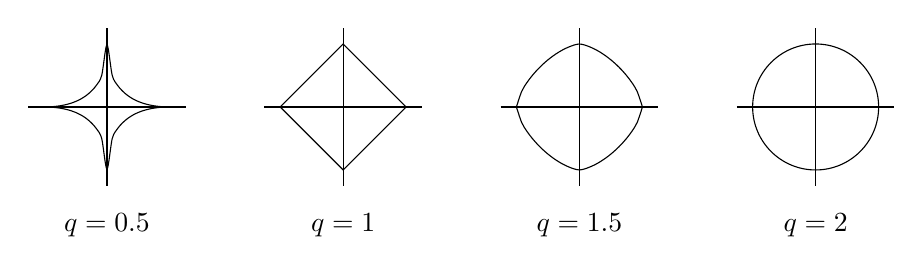
\begin{tikzpicture}
    \begin{scope}[shift={(0, 0)}]
      \draw (-1, 0) -- (1, 0);
      \draw (0, -1) -- (0, 1);
      \draw [domain=-0.8:0.8] plot [smooth] (\x, {(0.8^0.5 - (abs(\x))^0.5)^2});
      \draw [domain=-0.8:0.8] plot [smooth] (\x, {-(0.8^0.5 - (abs(\x))^0.5)^2});

      \node at (0, -1.5) {$q = 0.5$};
    \end{scope}
    \begin{scope}[shift={(3, 0)}]
      \draw (-1, 0) -- (1, 0);
      \draw (0, -1) -- (0, 1);
      \draw (0.8, 0) -- (0, 0.8) -- (-0.8, 0) -- (0, -0.8) -- cycle;

      \node at (0, -1.5) {$q = 1$};
    \end{scope}
    \begin{scope}[shift={(6, 0)}]
      \draw (-1, 0) -- (1, 0);
      \draw (0, -1) -- (0, 1);
      \draw [domain=-0.8:0.8] plot [smooth] (\x, {(0.8^1.5 - (abs(\x))^1.5)^(1/1.5)});
      \draw [domain=-0.8:0.8] plot [smooth] (\x, {-(0.8^1.5 - (abs(\x))^1.5)^(1/1.5)});

      \node at (0, -1.5) {$q = 1.5$};
    \end{scope}
    \begin{scope}[shift={(9, 0)}]
      \draw (-1, 0) -- (1, 0);
      \draw (0, -1) -- (0, 1);
      \draw circle [radius=0.8];

      \node at (0, -1.5) {$q = 2$};
    \end{scope}

  \end{tikzpicture}
\end{center}

We see that $q = 1$ is the smallest value of $q$ for which there are corners, and also the largest value of $q$ for which the constraint set is still convex. Thus, $q = 1$ is the sweet spot for doing regression.

\subsection{Prediction error with no design assumptions}
We suppose the columns of $X$ are scaled to have $\ell_2$ norm $\sqrt{n}$. We also assume that we have a normal linear model (after centering). Then
\[
  Y = X \beta^0 + \varepsilon- \bar{\varepsilon} 1,
\]
where $\varepsilon \sin N_n(0, \sigma^2 I)$.

\begin{thm}
  Let $\hat{\beta}$ be the Lasso solution when
  \[
    \lambda = A \sigma \sqrt{\frac{\log p}{n}}.
  \]
  With probability $1 - 2p^{-(A^2/2 - 1)}$, then
  \[
    \frac{1}{n} \|X \beta^0 - X \hat{\beta}\|_2^2 \leq 4A \sigma \sqrt{\frac{\log p}{n}} \|\beta^0\|_1.
  \]
\end{thm}
Crucially, this is proportional to $\log p$, and not just $p$. On the other hand, unlike what we usually see for ordinary least squares, we have $\frac{1}{\sqrt{n}}$, and not $\frac{1}{n}$. This is because we made no design assumptions.

\begin{proof}
  We don't really have a closed form solution for $\hat{\beta}$, and in general it doesn't exist. So the only thing we can use is that it in fact minimizes $Q_\lambda(\beta)$. Thus, by definition, we have
  \[
    \frac{1}{2n} \|Y - X \hat{\beta}\|_2^2 + \lambda \|\hat{\beta}\|_1 \leq \frac{1}{2n} \|Y - X \beta^0\|^2_2 + \lambda \|\beta^0\|_1.
  \]
  We know exactly what $Y$ is. It is $X \beta^0 + \varepsilon - \bar{\varepsilon} 1$. If we plug this in, we get
  \[
    \frac{1}{2n} \|X \beta^0 - X \hat{\beta}\|_2^2 \leq \frac{1}{n} \varepsilon^T X(\hat{\beta} - \beta^0) + \lambda \|\beta^0\|_1 - \lambda \|\hat{\beta}\|_1.
  \]
  Here we use the fact that $X$ is centered, and so is orthogonal to $1$.

  Now note that
  \[
    |\varepsilon^T X (\hat{\beta} - \beta^0)| \leq \|X^T \varepsilon \|_\infty \|\hat{\beta} - \beta^0\|_1.
  \]
  We'd like to bound $\|X^T \varepsilon \|_\infty$, but it can be arbitrarily large since $\varepsilon$ is a Gaussian. However, with high probability, it is small. Precisely, define
  \[
    \Omega = \left\{\frac{1}{n} \|X^T \varepsilon \|_\infty \leq \lambda\right\}.
  \]
  In a later lemma, we will show later that $\P(\Omega) \geq 1 - 2 p^{-(A^2/2 - 1)}$. We then work on $\Omega$, we have
  \begin{align*}
    \frac{1}{2n} \|X \beta^0 - X \hat{\beta}\|^2_2 &\leq \lambda \|\hat{\beta} - \beta^0\| - \lambda \|\hat{\beta}\| + \lambda \|\beta^0\|\\
    &\leq 2 \lambda \|\beta^0\|_1,
  \end{align*}
  where we used the triangle inequality in the last step. Then we are done.
\end{proof}

\subsubsection*{Basic concentration inequalities}
Consider the event $\Omega$. Then
\begin{align*}
  \P\left(\frac{1}{n} \|X^T \varepsilon\|_\infty > \lambda\right) &= \P\left(\bigcup_{j = 1}^p \left\{\frac{1}{n}|X_j^T \varepsilon| > \lambda\right\}\right)\\
  &\leq \sum_{j = 1}^p \P\left(\frac{1}{n} |X_j^T \varepsilon| > \lambda\right).
\end{align*}
Now $\frac{1}{n} X_j^T \varepsilon \sim N(0, \frac{\sigma^2}{n})$. So we just have to bound tail probabilities of normal random variables.

The simplest tail bound we have is Markov's inequality.
\begin{lemma}[Markov's inequality]\index{Markov's inequality}
  Let $W$ be a non-negative random variable. Then
  \[
    \P(W \geq t) \leq \frac{1}{t} \E W.
  \]
\end{lemma}

\begin{proof}
  We have
  \[
    t \mathbf{1}_{W \geq t} \leq W.
  \]
  The result then follows from taking expectations and then dividing both sides by $t$.
\end{proof}

While this is a very simply bound, it is rather useful. Given any strictly increasing function $\varphi: \R \to (0, \infty)$ and any random variable $W$, we have
\[
  \P(W \geq t) = \P(\varphi(W) \geq \varphi(t))\leq \frac{1}{\varphi(t)} \E \varphi(W).
\]
Applying this with $\varphi (t) = e^{\alpha t}$ for some $\alpha > 0$, we obtain the \term{Chernoff bound}:
\begin{cor}
  For any random variable $W$, we have
  \[
    \P(W \geq t) \leq \inf_{\alpha > 0} e^{-\alpha t} \E e^{\alpha W}.
  \]
\end{cor}
Note that $\E e^{\alpha W}$ is just the moment generating function of $W$, which we can compute quite straightforwardly.

We can immediately apply this when $W$ is a normal random variable, $W \sim N(0, \sigma^2)$. Then
\[
  \E e^{\alpha W} = e^{\alpha^2 \sigma^2/2}.
\]
So we have
\[
  \P(W \geq t) \leq \inf_{\alpha > 0}\exp \left(\frac{\alpha^2 \sigma^2}{2} - \alpha t\right) = e^{-t^2/(2\sigma^2)}.
\]
Observe that in fact this tail bound works for any random variable whose moment generating function is bounded above by $e^{\alpha^2 \sigma^2/2}$.

\begin{defi}[Sub-Gaussian random variable]\index{sub-Gaussian random variable}
  A random variable $W$ is \emph{sub-Gaussian} (with parameter $\sigma$) if
  \[
    \E e^{\alpha (W - \E W)} \leq e^{\alpha^2 \sigma^2/2}
  \]
  for all $\alpha \in \R$.
\end{defi}

\begin{cor}
  Any sub-Gaussian random variable $W$ with parameter $\sigma$ satisfies
  \[
    \P(W \geq t) \leq e^{-t^2/2\sigma^2}.\tag*{$\square$}
  \]
\end{cor}
Thus, our bound for the Lasso works also for sub-Gaussian random variables.

In general, bounded random variables are sub-Gaussian.
\begin{lemma}[Hoeffding's lemma]
  If $W$ has mean zero and takes values in $[a, b]$, then $W$ is sub-Gaussian with parameter $\frac{b - a}{2}$.\qedsym
\end{lemma}

Recall that the sum of two independent Gaussians is still a Gaussian. This continues to hold for sub-Gaussian random variables.

\begin{prop}
  Let $(W_i)_{i = 1}^n$ be a collection of independent mean-zero sub-Gaussian random variables with parameters $(\sigma_i)_{i = 0}^n$, and let $\gamma \in \R^n$. Then $\gamma^T W$ is sub-Gaussian with parameter
  \[
    \left(\sum (\gamma_i \sigma_i)^2\right)^{1/2}.
  \]
\end{prop}

\begin{proof}
  We have
  \begin{align*}
    \E \exp \left(\alpha \sum_{i = 1}^n \gamma_i W_i\right) &= \prod_{i = 1}^n \E \exp \left(\alpha \gamma_i W_i\right)\\
    &= \prod_{i = 1}^n \exp\left(\frac{\alpha^2}{2} \gamma_i^2 \sigma_i^2\right)\\
    &= \exp\left(\frac{\alpha^2}{2} \sum_{i = 1}^n \sigma_i^2 \gamma_i^2\right).\qedhere
  \end{align*}
\end{proof}

\begin{lemma}
  Suppose $(\varepsilon_i)_{i = 1}^n$ are independent, mean-zero sub-Gaussian with common parameter $\sigma$. Let
  \[
    \lambda = A \sigma \sqrt{\frac{\log p}{n}}.
  \]
  Let $X$ be a matrix whose columns all have norm $\sqrt{n}$. Then 
  \[
    \P\left(\frac{1}{n} \|X^T \varepsilon\|_{\infty} \leq \lambda\right) \geq 1 - 2p^{-(A^2/2 - 1)}. % define what X is.
  \]
\end{lemma}
In particular, this includes $\varepsilon \sim N_n(0, \sigma^2I)$.

\begin{proof}
  We have
  \[
    \P\left(\frac{1}{n}\|X^T \varepsilon\|_{\infty} > \lambda \right) \leq \sum_{j = 1}^p \P\left(\frac{1}{n} |X_j^T \varepsilon| > \lambda\right).
  \]
  But $\pm \frac{1}{n} X_j^T \varepsilon$ are both sub-Gaussian with parameter
  \[
    \sigma \left(\sum_i \left(\frac{X_{ij}}{n}\right)^2\right)^{1/2} = \frac{\sigma}{\sqrt{n}}.
  \]
  Then by our previous corollary, we get
  \[
    \sum_{j = 1}^p \P\left(\frac{1}{n} |X_j^T \varepsilon|_\infty > \lambda\right) \leq 2p \exp \left(- \frac{\lambda^2 n}{2\sigma^2}\right).
  \]
  Note that we have the factor of $2$ since we need to consider the two cases $\frac{1}{n} X_j^T \varepsilon > \lambda$ and $-\frac{1}{n} X_j^T \varepsilon > \lambda$.

  Plugging in our expression of $\lambda$, we write the bound as
  \[
    2p \exp\left(-\frac{1}{2} A^2 \log p\right) = 2p^{1 - A^2/2}.
  \]
\end{proof}
This is all we need for our result on the Lasso. We are going to go a bit further into this topic of concentration inequalities, because we will need them later when we impose conditions on the design matrix. In particular, we would like to bound the tail probabilities of products.

\begin{defi}[Bernstein's condition]\index{Bernstein's condition}
  We say that a random variable $W$ satisfies Bernstein's condition with parameters $(\sigma, b)$ where $a, b > 0$ if
  \[
    \E[|W - \E W|^k] \leq \frac{1}{2} k! \sigma^2 b^{k - 2}
  \]
  for $k = 2, 3, \ldots$.
\end{defi}
The point is that these bounds on the moments lets us bound the moment generating function of $W$.

\begin{prop}[Bernstein's inequality]\index{Bernstein's inequality}
  Let $W_1, W_2, \ldots, W_n$ be independent random variables with $\E W_i = \mu$, and suppose each $W_i$ satisfies Bernstein's condition with parameters $(\sigma, b)$. Then
  \[
    \E e^{\alpha(W_i - \mu)} \leq \exp \left(\frac{\alpha^2 \sigma^2/2}{1 - b|\alpha|}\right)
  \]
  for $|\alpha| < \frac{1}{b}$. Moreover,
  \[
    \P\left(\frac{1}{n} \sum_{i = 1}^n W_i - \mu \geq t\right) \leq \exp \left(-\frac{nt^2}{2 (\sigma^2 + bt)}\right)
  \]
  for all $t \geq 0$
\end{prop}
Note that for large $t$, the bound goes as $e^{-t}$ instead of $e^{-t^2}$.

\begin{proof}
  For the first part, we fix $i$ and write $W = W_i$. Let $|\alpha| < \frac{1}{n}$. Then
  \begin{align*}
    \E e^{\alpha(W_i - \mu)} &= \sum_{i = 0}^\infty \E \frac{1}{k!} \alpha^k |W_i - \mu|^k\\
    &\leq 1 + \frac{\sigma^2 \alpha^2}{2} |\alpha|^{k - 2} b^{k - 2}\\
    &= 1 + \frac{\sigma^2 \alpha^2}{2} \frac{1}{1 - |\alpha|b}\\
    &\leq \exp \left(\frac{\alpha^2 \sigma^2/2}{1 - b|\alpha|}\right).
  \end{align*}
  Then
  \begin{align*}
    \E \exp\left(\frac{1}{n} \sum_{i = 1}^n \alpha (W_i - \mu)\right) &= \prod_{i = 1}^n \E \exp\left(\frac{\alpha}{n} (W_i - \mu)\right)\\
    &\leq \exp \left(n \frac{\left(\frac{\alpha}{n}\right)^2 \sigma^2/2}{1 - b \left|\frac{\alpha}{n}\right|}\right),
  \end{align*}
  assuming $\left|\frac{\alpha}{n}\right| < \frac{1}{n}$.  So it follows that
  \[
    \P \left(\frac{1}{n} \sum_{i = 1}^n W_i - \mu \geq t\right) \leq e^{-\alpha t}.
  \]
  Setting
  \[
    \frac{\alpha}{n} = \frac{t}{bt + \sigma^2} \in \left[0, \frac{1}{b}\right)
  \]
  gives the result.
\end{proof}

\begin{lemma}
  Let $W, Z$ be mean-zero sub-Gaussian random variables with parameters $\sigma_W$ and $\sigma_Z$ respectively. Then $WZ$ satisfies Bernstein's condition with parameter $(8 \sigma_W \sigma_Z, 4 \sigma_W \sigma_Z)$.
\end{lemma}

\begin{proof}
  For any random variable $Y$ (which we will later take to be $WZ$), for $k > 1$, we know
  \begin{align*}
    \E |Y - \E Y|^k &= 2^k \E \left| \frac{1}{2}Y - \frac{1}{2}\E Y\right|^k\\
    &\leq 2^k \E \left| \frac{1}{2} |Y| + \frac{1}{2} |\E Y|\right|^k.
  \end{align*}
  Note that
  \[
    \left| \frac{1}{2} |Y| + \frac{1}{2} |\E Y|\right|^k \leq \frac{|Y|^k + |\E Y|^k}{2}
  \]
  by Jensen's inequality. Applying Jensen's inequality again, we have
  \[
    |\E Y|^k \leq \E |Y|^k.
  \]
  Putting the whole thing together, we have
  \[
    \E |Y - \E Y|^k \leq 2^k \E |Y|^k.
  \]
  Now take $Y = WZ$. Then
  \[
    \E |WZ - \E WZ| \leq 2^k \E |WZ|^k \leq 2^k \left(\E W^{2k}\right)^{1/2} (\E Z^{2k})^{1/2},
  \]
  by the Cauchy--Schwarz inequality.

  We know that sub-Gaussians satisfy a bound on the tail probability. We can then use this to bound the moments of $W$ and $Z$. First note that
  \[
    W^{2k} = \int_0^\infty \mathbf{1}_{x < W^{2k}} \;\d x.
  \]
  Taking expectations of both sides, we get
  \[
    \E W^{2k} = \int_0^\infty \P(x < W^{2k})\;\d x.
  \]
  Since we have a tail bound on $W$ instead of $w^{2k}$, we substitute $x = t^{2k}$. Then $\d x = 2k t^{2k - 1}\;\d t$. So we get
  \begin{align*}
    \E W^{2k} &= 2k \int_0^\infty t^{2k - 1} \P(|W| > t) \;\d t\\
    &= 4k \int_0^\infty t^{2k} \exp \left(-\frac{t^2}{2 \sigma_N^2}\right)\;\d t.
  \end{align*}
  where again we have a factor of $2$ to account for both signs. We perform yet another substitution
  \[
    x = \frac{t^2}{2 \sigma_N^2},\quad \d x = \frac{t}{\sigma_W^2}\;\d t.
  \]
  Then we get
  \[
    \E W^{2k} = 2^{k + 1} \sigma_W^{2k} k \sigma_W^2 \int_0^\infty x^{k - 1} e^{-x}\;\d x = 4 \cdot k! \sigma_W^2.
  \]
  Then we are done.
\end{proof}

\printindex
\end{document}
